\section{Cahier des charges}\label{cahier-des-charges}

\subsection{Site}\label{site}

Chaque site consiste en une grille carrée de \texttt{TAILLE\_TERRAIN}
cases de côté. Au centre de chaque bord se trouve une rangée de bases de
\texttt{LONGUEUR\_BASE} cases, encadrée de zones interdites de chaque
côté. Le reste de la région est constitué de pulsars et de cases vides.

\noindent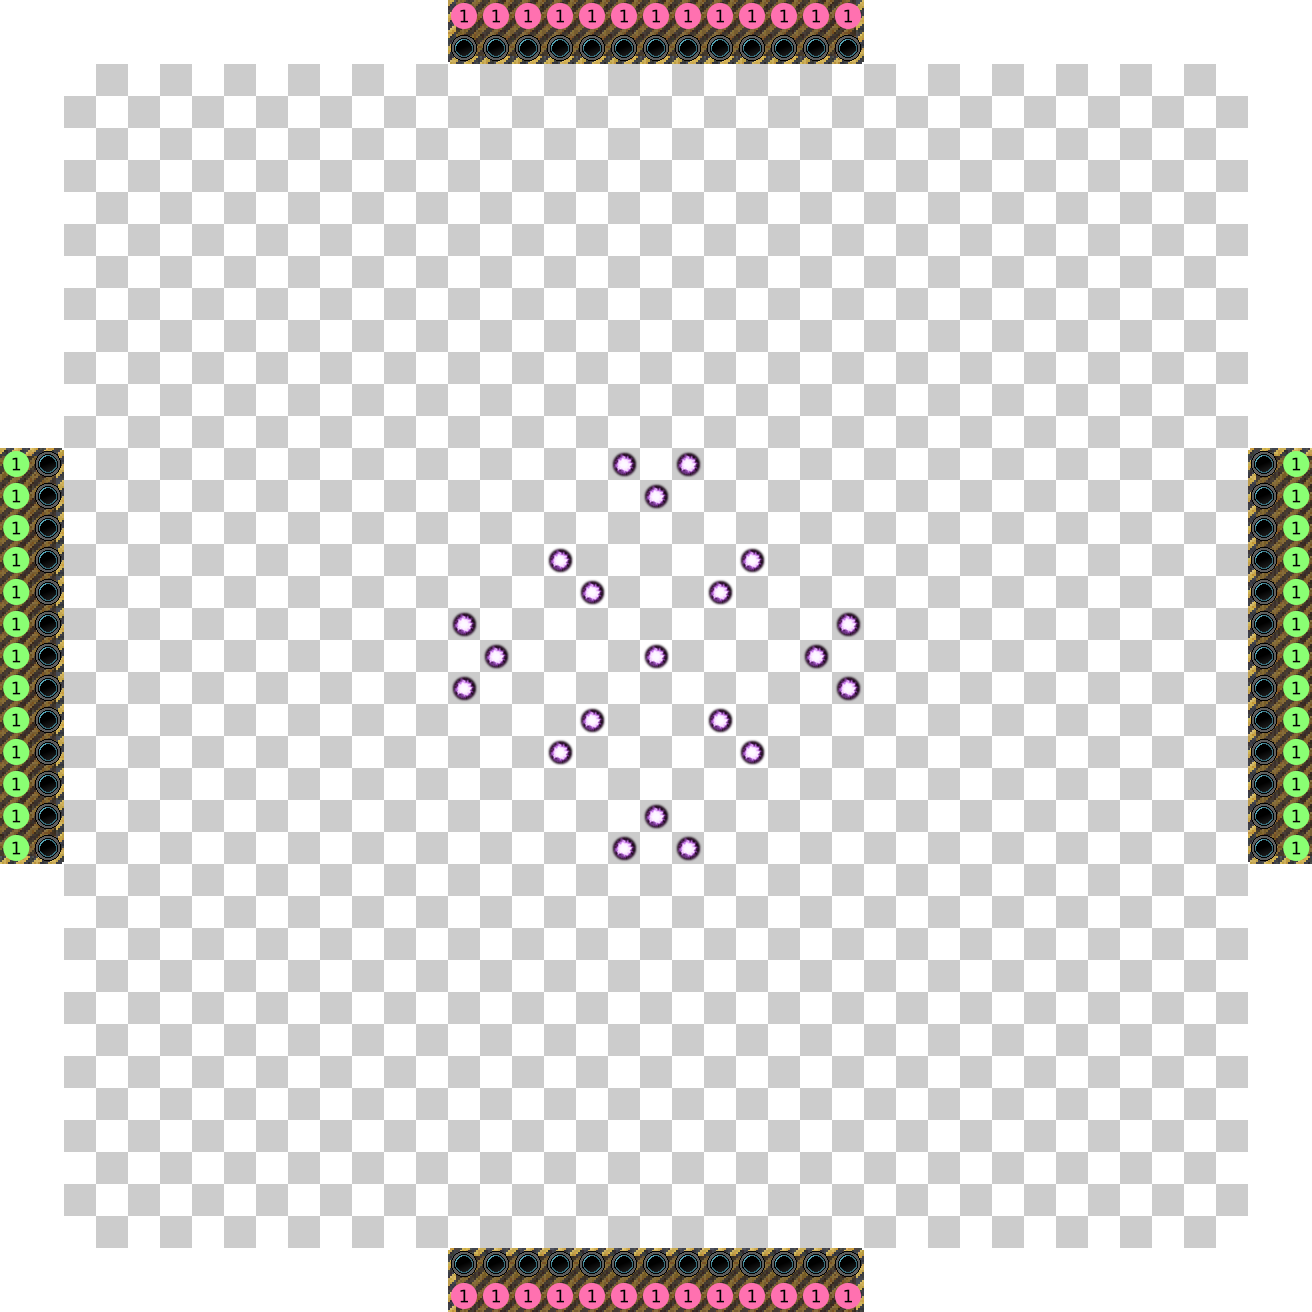
\includegraphics[width=\textwidth]{asset/site.png}

\subsubsection{Base}\label{base}

Les bases se trouvant sur deux bords opposés appartiennent au même
joueur. Chaque case possède initialement une unité de puissance
d'aspiration, qui pourra être assignée à d'autres cases en cours de jeu,
dans la limite de \texttt{LIMITE\_ASPIRATION} unités par case.

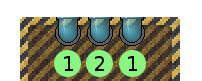
\includegraphics{asset/base.png}

{Trois cases de base (au sud) de puissance d'aspiration 1, 2 et 1.}

\subsubsection{Zone interdite}\label{zone-interdite}

Ce sont les cases du bord des sites qui ne sont pas des cases de base,
il n'est pas possible de construire par dessus.


\includegraphics{asset/interdit.png}

{La zone interdite, en rouge, de part et d'autre d'une base (au sud) de taille 3 sur un site de côté 9.}

\subsubsection{Vide}\label{vide}

Ce sont des cases qui ne contiennent rien, la seule action possible est
de construire par dessus.


\includegraphics{asset/vide.png}

{Du vide entre deux tuyaux.}

\subsubsection{Pulsar}\label{pulsar}

Un pulsar a une position fixe, et possède des caractéristiques qui lui
sont propres :

\begin{itemize}
\tightlist
\item
  une période de pulsation \emph{T};
\item
  une puissance de pulsation \emph{P};
\item
  un nombre de pulsations restantes \emph{R}.
\end{itemize}


\includegraphics{asset/pulsar.png}

{Un pulsar.}

\subsubsection{Tuyau}\label{tuyau}

Le tuyau est un composant qui permet de transporter le plasma. Les
effets d'un tuyau (ou d'un Super-Tuyau™) ne dépendent pas du joueur qui
l'a construit.


\includegraphics{asset/tuyau.png}

{Trois tuyaux.}

\subsubsection{Super-Tuyau™}\label{super-tuyau}

Le Super-Tuyau™ transporte du plasma plus rapidement qu'un tuyau et
coûte plus cher à détruire.


\includegraphics{asset/supertuyau.png}

{Un SuperTuyau™ entre deux tuyaux.}

\subsubsection{Débris}\label{duxe9bris}

Ce sont les restes de la destruction d'un tuyau. Du plasma peut en
sortir mais pas y rentrer.


\includegraphics{asset/debris.png}

{Un débris entre deux tuyaux.}

\subsection{Déroulement d'un tour}\label{duxe9roulement-dun-tour}

Au début de votre tour, vous recevez \texttt{NB\_POINTS\_ACTION}
\emph{points d'action} valables pour ce tour seulement. Ils vous
permettent d'effectuer les actions ci-dessous.

\subsubsection{Actions}\label{actions}

\paragraph{Construire un tuyau}\label{construire-un-tuyau}

Vous pouvez dépenser \texttt{COUT\_CONSTRUCTION} points d'action pour
construire un tuyau sur une case vide.

\paragraph{Améliorer un tuyau en
Super-Tuyau™}\label{amuxe9liorer-un-tuyau-en-super-tuyau}

Vous pouvez dépenser \texttt{COUT\_AMELIORATION} points d'action pour
améliorer un tuyau existant en Super-Tuyau™.

\paragraph{Détruire un tuyau}\label{duxe9truire-un-tuyau}

Vous pouvez dépenser \texttt{COUT\_DESTRUCTION} points d'action pour
lancer un \emph{tir de plasma} et détruire un tuyau, ou
\texttt{COUT\_DESTRUCTION\_SUPER\_TUYAU} points d'action pour détruire
un Super-Tuyau™. Un tir de plasma vous consomme de plus
\texttt{CHARGE\_DESTRUCTION} charges de plasma que vous avez collecté.
La case visée est remplacée par une case de débris.

Le plasma encore présent dans le tuyau ou Super-Tuyau™ détruit persiste
dans les débris.

\paragraph{Déblayer des débris}\label{duxe9blayer-des-duxe9bris}

Vous pouvez dépenser \texttt{COUT\_DEBLAYAGE} points d'action pour
déblayer des débris, rendant la case vide.

\paragraph{Modifier la puissance
d'aspiration}\label{modifier-la-puissance-daspiration}

Cette action est gratuite une fois par tour, et coûte ensuite
\texttt{COUT\_MODIFICATION\_ASPIRATION} points d'action à refaire dans
le même tour.

Vous déplacez une unité de puissance d'aspiration d'une de vos cases de
base à une autre (éventuellement sur le bord opposé). Bien sûr, vous ne
pouvez effectuer cette action que si la première case possède au moins
une unité.

\subsubsection{Plasma}\label{plasma}

Les pulsars sur la carte pulsent régulièrement du plasma que vous devez
acheminer à votre base avec des tuyaux pour l'extraire et augmenter
votre score. La quantité de plasma se mesure en \emph{charges}, un
nombre réel positif.

À la fin du tour de chaque joueur, le plasma présent sur la carte se
déplace en direction des bases les plus proches.

Le plasma dans des tuyaux qui ne sont reliés à aucune base par d'autres
tuyaux disparaît définitivement. Sinon, les règles ci-dessous
s'appliquent.

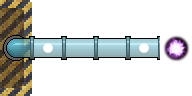
\includegraphics{asset/debris_t0.png}\hfill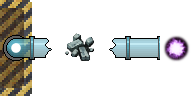
\includegraphics{asset/debris_t1.png}

\begin{itemize}
\item $t_0$ : du plasma dans un tuyau en direction de la base.
\item $t_1$ : un joueur a détruit un tuyau, le plasma qui n'est pas encore arrivé
dans la base est donc perdu.
\end{itemize}

La \emph{distance effective} entre une case \texttt{c} et une case de
base \texttt{b} est égale à \texttt{D(c,b)-A(b)}, où \texttt{D(c,b)} est
la longueur du plus court chemin de \texttt{c} à \texttt{b} ne passant
que par des tuyaux et \texttt{A(b)} est la puissance d'aspiration
possédée par la case \texttt{b}. Un Super-Tuyau™ est considéré comme un
tuyau dans le calcul des distances. La \emph{distance minimale} d'une
case est la plus petite distance effective entre cette case et n'importe
quelle case de base à laquelle elle est reliée.

\noindent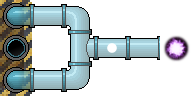
\includegraphics[width=0.3\textwidth]{asset/split_t0.png}\hfill
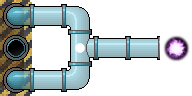
\includegraphics[width=0.3\textwidth]{asset/split_t1.png}\hfill
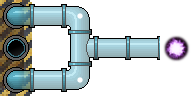
\includegraphics[width=0.3\textwidth]{asset/split_t2.png}

Déplacement du plasma à une intersection. Toutes les bases ont la même
puissance d'aspiration.

À la fin d'un tour, il peut y avoir du plasma dans un tuyau, un
Super-Tuyau™, ou des débris. À partir d'une case à distance minimale
\texttt{D\_min}, le plasma se déplace vers les cases voisines de base,
tuyau ou Super-Tuyau™ à distance minimale \texttt{D\_min-1}. Il y en a
toujours au moins une. Quand il y en a plusieurs, le plasma se divise en
quantités égales sur chacune de ces cases. Le plasma qui arrive sur une
case de base est immédiatement collecté par le joueur propriétaire de
cette case.

Le plasma avance d'une case s'il se trouve initialement sur un tuyau ou
des débris, deux sur un Super-Tuyau™, sans être affecté par d'autres
Super-Tuyaux™ sur son trajet.

\noindent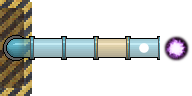
\includegraphics[width=0.3\textwidth]{asset/super_t0.png}\hfill
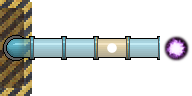
\includegraphics[width=0.3\textwidth]{asset/super_t1.png}\hfill
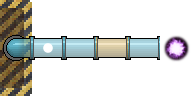
\includegraphics[width=0.3\textwidth]{asset/super_t2.png}

Déplacement du plasma dans un SuperTuyau™.


Enfin, quand la période d'un pulsar \texttt{T} est un diviseur du nombre
de tours passés et qu'il lui reste des pulsations
(\texttt{R\ \textgreater{}\ 0}), il pulse, ce qui décrémente \texttt{R}
et ajoute \texttt{P} charges de plasma à chacune des quatre cases
adjacentes au pulsar. Ce plasma disparaît immédiatement s'il ne se
trouve pas dans un tuyau relié à une base.

\subsubsection{Score}\label{score}

Votre score est la quantité de plasma que vous avez collecté, arrondie à
l'entier inférieur. Détruire un tuyau vous coûte du plasma, ce qui
réduit effectivement votre score.

\subsubsection{Format de la carte}\label{format-de-la-carte}

La carte est donnée par un fichier texte, où chaque ligne donne les
caractéristiques d'un pulsar sur la carte, sous la forme de cinq entiers
: \emph{abscisse}, \emph{ordonnée}, \emph{période}, \emph{puissance},
\emph{nombre total de pulsations}.

Voici un exemple avec deux pulsars :

\begin{verbatim}
11 15 9 5 8
15 11 9 5 8
\end{verbatim}
